\documentclass[12pt, a4paper, twoside, openright]{report}
\usepackage[colorlinks=true, linkcolor=black, citecolor=black, urlcolor=black]{hyperref}

\input{preamble.tex}
\setlength{\parindent}{0pt}

% ============= Document ============= %
\begin{document}

% =========== Frontespizio =========== %
\input{frontespizio}
\blankpage
\blankpage
\restoregeometry

% ============== Indice ============== %
\pagenumbering{roman}
\tableofcontents
\listoffigures
%\listoftables
%\lstlistoflistings
\afterpage{\blankpage}
\newpage
\pagenumbering{arabic}

% ============= Capitoli ============= %
\chapter{Iterazione 0}
\section{Introduzione}

OptiTour è un'app che ottimizza gli itinerari turistici calcolando automaticamente il percorso più efficiente per visitare una serie di luoghi nel tempo a disposizione.

Scegliere cosa visitare è semplice, ma organizzare le tappe nell'ordine migliore richiede tempo, esperienza e una valutazione accurata dei tempi di spostamento e di visita. A differenza delle comuni app di mappe, OptiTour non si limita a mostrare i punti di interesse, ma trasforma una lista di monumenti in un itinerario ottimale.

L'utente seleziona il punto di partenza e i luoghi che desidera visitare, indicando quanto tempo ha a disposizione. L'app, elaborando queste informazioni, dà origine al percorso più rapido, garantendo che l'itinerario rispetti la finestra temporale impostata.

\vspace{9pt}
Con OptiTour, l'utente può:
\begin{itemize}
    \item \textbf{Pianificazione Itinerari Smart:} selezione dei punti di interesse (POI) e calcolo del ciclo ottimale per ridurre chilometri e tempi di percorrenza.
    \item \textbf{Gestione Flessibile:} possibilità di creare nuovi viaggi (manuali o casuali), modificare le tappe, visualizzare dettagli o eliminare percorsi.
    \item \textbf{Social e Storico:} salvataggio dei percorsi preferiti, consultazione dello storico dei viaggi effettuati, condivisione e aggiunta di recensioni.
    \item \textbf{Gestione Profilo:} registrazione, login e gestione sicura dei dati personali e delle credenziali.
\end{itemize}

L'applicazione si interfaccia direttamente con provider di servizi geografici esterni per garantire che il calcolo delle distanze e dei tempi sia basato su dati reali e aggiornati.

\vspace{1cm}

\textbf{Perché scegliere OptiTour?}

\medskip

OptiTour nasce per rispondere a un'esigenza specifica: l'efficienza nella programmazione di itinerari. Spesso i turisti perdono tempo prezioso camminando avanti e indietro per la città a causa di una pianificazione non ottimale o assente. Questo problema, noto come \textit{Traveling Salesman Problem} (TSP), diventa difficile da risolvere mentalmente man mano che il numero di luoghi da visitare aumenta.

OptiTour automatizza questo processo complesso utilizzando algoritmi avanzati sui grafi ed euristiche dedicate. Il sistema non offre solo un percorso, ma il miglior percorso possibile, rendendolo lo strumento ideale per diverse tipologie di utenti: dal turista che vuole massimizzare le visite nel tempo a disposizione, allo sportivo che cerca un percorso di allenamento circolare che tocchi specifici punti di interesse, fino ai professionisti dell'ospitalità che desiderano offrire itinerari personalizzati ai propri ospiti.

Con un'interfaccia intuitiva che separa nettamente la logica di presentazione da quella algoritmica, OptiTour offre una soluzione potente ma accessibile per trasformare il modo in cui esploriamo le città.
\newpage
\input{Iterazione0/Requisiti.tex}
\newpage
\section{Casi D'uso}
\begin{figure}[H]
    \centering
    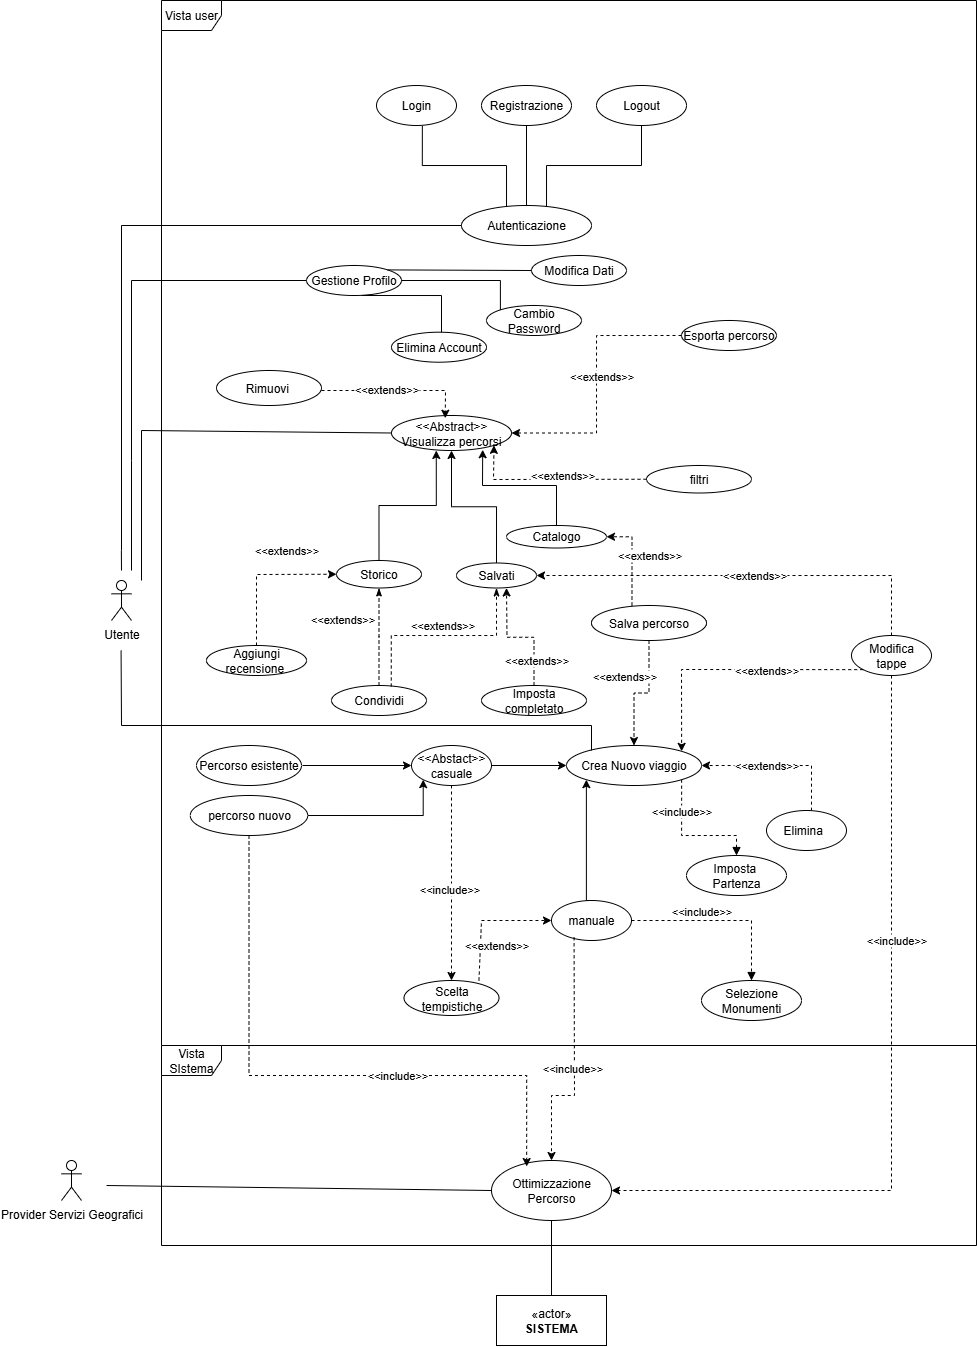
\includegraphics[width=0.8\textwidth]{Iterazione0/Diagrammi/DiagrammaCasiDusoV1.png}
    \caption{Casi d'uso}
    \label{fig:casi_d_uso}
\end{figure}    

Di seguito sono riportati i casi d’uso relativi al sistema di gestione percorsi e viaggi.
\begin{itemize}
  
    \item \textbf{UC1 - Autenticazione} 
 \begin{itemize}
  \item \textbf{UC1.1 - Registrazione:} un nuovo utente può creare un account personale fornendo i dati richiesti.

    \item \textbf{UC1.2 - Login:} un utente registrato può accedere al proprio account inserendo le proprie credenziali per iniziare una sessione e usare le funzionalità del sistema.

    \item \textbf{UC1.3 - Logout:} l’utente può terminare la propria sessione in modo sicuro.
\end{itemize}
    \item \textbf{UC2 - Gestione profilo}\begin{itemize}
   \item \textbf{UC2.1 - Modifica dati:} l'utente può modificare i propri dati personali in caso di neccessità.
    \item \textbf{UC2.2 - Elimina account:} l'utente può eliminare definitivamente il proprio account.
\end{itemize}


    \item \textbf{UC3 - Visualizza percorsi:} l'utente può visualizzare i dettagli di un percorso.
\begin{itemize}
    \item \textbf{UC3.1 - Catalogo:} è possibile visualizzare percorsi creati da altri utenti e inseriti in un catalogo.
    \item \textbf{UC3.2 - Salvati:} è possibile visualizzare percorsi provenienti dall’elenco dei percorsi salvati.
    \item \textbf{UC3.3 - Storico:} è possibile visualizzare percorsi provenienti dallo storico dei percorsi effettuati.
\end{itemize}

    \item \textbf{UC4 - Filtri ricerca:} l'utente può filtrare i percorsi in base a diversi criteri.

    \item \textbf{UC5 - Salva percorso:} l'utente può salvare un percorso nella sezione dei percorsi preferiti.

    \item \textbf{UC6 - Esporta percorso:} l'utente può esportare un percorso in un formato condivisibile.

    \item \textbf{UC7 - Rimuovi percorso salvato:} l'utente può rimuovere un percorso dai percorsi salvati.

    \item \textbf{UC8 - Condividi percorso:} l'utente può condividere un percorso con altri utenti.

    \item \textbf{UC9 - Aggiungi recensione:} l'utente può aggiungere una recensione a un percorso che è satao effettuato.

    \item \textbf{UC10 - Imposta percorso completato:} l'utente può contrassegnare un percorso come completato.

    \item \textbf{UC11 - Imposta punto di partenza:} l'utente seleziona il punto da cui far partire e finire il percorso.

    \item \textbf{UC12 - Crea nuovo viaggio:} 
\begin{itemize}
     \item \textbf{UC12.1 - Manuale:} l'utente può far creare il proprio percorso scegliendo autonomamente le tappe da visitare.
 \item \textbf{UC12.2 - Casuale:} 
\begin{itemize}
   \item \textbf{UC12.2.1 - Percorso esistente:} l'utente fa scegliere al sistema in modo casuale un percorso già esistente nel catalogo.
    \item \textbf{UC12.2.2 - Percorso nuovo:} l'utente fa generare al sistema in modo casuale un nuovo percorso.
\end{itemize}
\end{itemize} 

    \item \textbf{UC13 - Scelta tempistiche:} l'utente può definire le tempistiche del viaggio.

    \item \textbf{UC14 - Ottimizzazione percorso:} il sistema ottimizza tramite un algoritmo specifico l’ordine delle tappe.

    \item \textbf{UC15 - Modifica tappe:} l'utente può modificare le tappe di un percorso.

    \item \textbf{UC16 - Elimina tappa:} l'utente può eliminare una tappa dal percorso.
\end{itemize}
\input{Iterazione0/Deployment.tex}
\input{Iterazione0/Architettura.tex}
\input{Iterazione0/priorità.tex}
%\newpage
\input{Iterazione0/Topologia.tex}
\newpage
\section{Strumenti utilizzati}

Di seguito vengono illustrati gli strumenti e le tecnologie adottate per la realizzazione
del progetto. La scelta dello stack tecnologico è stata orientata a garantire la massima
integrazione tra la gestione dei dati geografici e un’architettura di tipo modulare.

\begin{itemize}

\item \textbf{Spring Boot:} Framework Java basato sull’ecosistema Spring, impiegato per implementare
la logica di backend secondo il pattern architetturale MVC. Spring Boot
facilita la gestione del Controller e l’integrazione del Model con i database, automatizzando
la configurazione dell’infrastruttura. Questo approccio garantisce una
chiara separazione delle responsabilità, rendendo l’applicazione scalabile, modulare
e facilmente manutenibile.

\item \textbf{GraphHopper:} motore di routing utilizzato per ottenere dati reali di distanza e
tempo di percorrenza tra le coordinate GPS dei punti di interesse. Fornisce la
componente pratica necessaria per calcolare percorsi realistici sulle strade esistenti,
garantendo itinerari ottimizzati basati su tempi reali di percorrenza e condizioni
stradali.

\item \textbf{JUnit 4:} Framework per il testing unitario in Java, impiegato per validare il corretto
funzionamento delle classi e dei metodi sviluppati. L’uso di test automatizzati
consente di rilevare tempestivamente eventuali errori e di garantire la robustezza del
codice.

\item \textbf{MongoDB e MongoDB Compass:} MongoDB è il database NoSQL utilizzato per
memorizzare i POI (Points of Interest) con strutture flessibili e attributi variabili
provenienti da OpenStreetMap, come nome, descrizione, coordinate, categorie e
immagini. Spring Data MongoDB facilita le operazioni CRUD e le query complesse.
MongoDB Compass, invece, è lo strumento grafico che permette di esplorare
visivamente le collezioni, verificare la correttezza dei documenti JSON e correggere
manualmente eventuali dati errati, migliorando il controllo sulla qualità dei dati.

\item \textbf{OpenStreetMap:} piattaforma open-source che fornisce dati geospaziali dettagliati.
I dati di OpenStreetMap sono utilizzati da Nominatim per il geocoding, da Overpass
API per interrogazioni sui monumenti e da React-Leaflet per la visualizzazione
delle mappe interattive nel frontend. La natura collaborativa di OpenStreetMap
garantisce dati aggiornati e accurati per il calcolo dei percorsi.

\item \textbf{Nominatim:} servizio di geocoding utilizzato per trasformare indirizzi testuali inseriti
dall’utente in coordinate geografiche precise ($lat/lon$), consentendo di posizionare
correttamente il punto di partenza dei percorsi sulla mappa.

\item \textbf{Overpass API:} interroga il database OpenStreetMap per individuare monumenti e
POI nelle vicinanze del punto di interesse indicato dall’utente. Per evitare di sovraccaricare
il servizio e garantire tempi di risposta rapidi, i dati vengono memorizzati
localmente su MongoDB dopo la prima richiesta, rendendo più efficienti le ricerche
successive.

\item \textbf{React.js \& Node.js:} React gestisce lo stato dell’interfaccia utente, come la lista dei
monumenti selezionati e le informazioni sul percorso ottimizzato, mentre Node.js
offre l’ambiente di esecuzione e la gestione dei pacchetti tramite npm. Insieme,
permettono di costruire un frontend dinamico, reattivo e facilmente aggiornabile.

\item \textbf{React-Leaflet:} libreria che connette React alle mappe interattive di OpenStreetMap.
Consente di posizionare marker sui monumenti, visualizzare linee di percorso ottimizzate
calcolate dal backend e rendere l’esperienza dell’utente più intuitiva grazie
a mappe dinamiche e interattive.

\item \textbf{Axios:} libreria per gestire chiamate HTTP asincrone. Permette al frontend di inviare
richieste al backend e ricevere le risposte in formato JSON senza ricaricare la pagina,
garantendo un’esperienza utente fluida e immediata.

\item \textbf{Eclipse:} IDE principale per la scrittura del codice Java, il debugging del backend e
la gestione del progetto tramite Maven o Gradle. Offre strumenti avanzati di refactoring,
analisi del codice e integrazione con sistemi di versionamento, migliorando
l’efficienza dello sviluppo.

\item \textbf{CodeMR:} strumento di analisi statica del codice sorgente, che estrae metriche di
coesione e accoppiamento delle classi. Aiuta a identificare classi troppo complesse
e suggerisce possibili rifattorizzazioni, migliorando la manutenibilità del software.

\item \textbf{Postman:} Strumento essenziale per il testing delle API REST sviluppate con Spring
Boot. Consente di effettuare richieste HTTP, validare le risposte del server e automatizzare
test, facilitando così il debug e l’integrazione tra i diversi componenti
del sistema.

\item \textbf{StarUML \& Diagrams.net:} strumenti utilizzati per la modellazione dei sistemi.
StarUML serve per diagrammi formali (casi d’uso, classi, deployment), mentre
Diagrams.net è utile per schemi logici, flussi di dati e rappresentazioni più informali,
favorendo la chiarezza della progettazione.

\item \textbf{GitHub \& GitHub Desktop:} strumenti di controllo di versione che permettono
di salvare lo storico dei file, gestire branch multipli e sincronizzare il lavoro tra
diversi membri del team, garantendo una collaborazione efficiente e tracciabilità
delle modifiche.

\item \textbf{WhatsApp:} applicazione di messaggistica utilizzata come strumento di comunicazione
interna tra i membri del team. Consente di coordinare le attività di sviluppo,
discutere problemi tecnici e organizzare riunioni in tempo reale, garantendo un
flusso comunicativo rapido ed efficiente.

\end{itemize}

\chapter{Iterazione 1}
\section{Casi d'uso implementati}
In questa fase sono stati sviluppati i seguenti casi d'uso ritenuti prioritari per lo sviluppo di OptiTour.

\begin{table}[hbt!]
    \centering
    \begin{tabular}{ll}
        \hline
        \textbf{ID} & \textbf{Titolo} \\
        \hline
        UC1.1 & Registrazione \\
        UC1.2 & Login \\
        UC1.3 & Logout \\
        UC11 & Imposta punto di partenza \\
        UC12.1 & Creazione itinerario manuale \\
        UC13 & Scelta tempistiche \\
        UC3 & Visualizza percorsi \\
        UC16 & Elimina viaggio \\
        UC14 & Ottimizzazione percorso \\
        \hline
    \end{tabular}
    \caption{Iterazione 1}
\end{table}

\subsection*{UC1.1: Registrazione}
\textbf{Attori:} Utente, Sistema. \\
\textbf{Descrizione:} Un nuovo utente può creare un account personale fornendo i dati richiesti. \\
\textbf{Flusso degli eventi:}
\begin{enumerate}
    \setlength{\itemsep}{0pt}
    \setlength{\parskip}{0pt}
    \item L'utente accede alla pagina di registrazione.
    \item Inserisce i propri dati personali e le credenziali.
    \item Il sistema verifica i dati e crea il nuovo account.
    \item L'utente viene reindirizzato alla pagina di login.
\end{enumerate}

\subsection*{UC1.2: Login}
\textbf{Attori:} Utente, Sistema. \\
\textbf{Descrizione:} Un utente registrato può accedere al proprio account inserendo le proprie credenziali. \\
\textbf{Flusso degli eventi:}
\begin{enumerate}
    \setlength{\itemsep}{0pt}
    \setlength{\parskip}{0pt}
    \item L'utente accede alla pagina di login.
    \item Inserisce email e password.
    \item Il sistema verifica le credenziali e autentica l'utente.
    \item L'utente viene reindirizzato alla home.
\end{enumerate}

\subsection*{UC1.3: Logout}
\textbf{Attori:} Utente, Sistema. \\
\textbf{Descrizione:} L'utente può terminare la propria sessione in modo sicuro. \\
\textbf{Flusso degli eventi:}
\begin{enumerate}
    \setlength{\itemsep}{0pt}
    \setlength{\parskip}{0pt}
    \item L'utente clicca sul pulsante di logout.
    \item Il sistema termina la sessione corrente.
    \item L'utente viene reindirizzato alla pagina di login.
\end{enumerate}

\subsection*{UC11: Imposta punto di partenza}
\textbf{Attori:} Utente, Sistema \\
\textbf{Descrizione:} L'utente inserisce un indirizzo testuale come punto di partenza del viaggio. Il sistema converte automaticamente l'indirizzo in coordinate geografiche tramite il servizio esterno Nominatim e le salva nel viaggio. \\
\textbf{Flusso degli eventi:}
\begin{enumerate}
    \setlength{\itemsep}{0pt}
    \setlength{\parskip}{0pt}
    \item L'utente inserisce un indirizzo di partenza nel campo apposito.
    \item Il sistema invia l'indirizzo al servizio Nominatim.
    \item Nominatim restituisce le coordinate geografiche corrispondenti.
    \item Le coordinate vengono salvate nel viaggio e la mappa si aggiorna sul punto selezionato.
\end{enumerate}

\subsection*{UC12.1: Creazione itinerario manuale}
\textbf{Attori:} Utente, Sistema. \\
\textbf{Descrizione:} L'utente seleziona manualmente i monumenti che desidera visitare. I monumenti vengono recuperati da Overpass API la prima volta e salvati in MongoDB per evitare chiamate ripetute al servizio esterno. \\
\textbf{Flusso degli eventi:}
\begin{enumerate}
    \setlength{\itemsep}{0pt}
    \setlength{\parskip}{0pt}
    \item L'utente cerca i monumenti di una città.
    \item Il sistema verifica se i monumenti sono già presenti in MongoDB.
    \item Se non presenti, il sistema li recupera tramite Overpass API e li salva nel database.
    \item I monumenti vengono mostrati sulla mappa.
    \item L'utente seleziona i monumenti che desidera visitare.
    \item L'utente conferma la selezione e il sistema salva il viaggio.
\end{enumerate}

\subsection*{UC13: Scelta tempistiche}
\textbf{Attori:} Utente, Sistema. \\
\textbf{Descrizione:} L'utente può definire per ciascun monumento selezionato il tempo che intende dedicare alla visita, espresso in minuti. \\
\textbf{Flusso degli eventi:}
\begin{enumerate}
    \setlength{\itemsep}{0pt}
    \setlength{\parskip}{0pt}
    \item L'utente seleziona un monumento durante la creazione del viaggio.
    \item Inserisce il tempo di visita desiderato in minuti.
    \item Il sistema salva il tempo di visita associato a quella tappa del viaggio.
\end{enumerate}

\subsection*{UC3.2: Visualizza percorsi}
\textbf{Attori:} Utente, Sistema. \\
\textbf{Descrizione:} L'utente può visualizzare i propri viaggi e di visualizzare i dettagli del singolo viaggio. \\
\textbf{Flusso degli eventi:}
\begin{enumerate}
    \setlength{\itemsep}{0pt}
    \setlength{\parskip}{0pt}
    \item L'utente accede alla sezione dei propri viaggi.
    \item Il sistema recupera tutti i viaggi dell'utente dal database.
    \item L'utente può selezionare un singolo viaggio per visualizzarne i dettagli.
\end{enumerate}

\subsection*{UC16: Elimina viaggio}
\textbf{Attori:} Utente, Sistema. \\
\textbf{Descrizione:} L'utente può eliminare un viaggio esistente. \\
\textbf{Flusso degli eventi:}
\begin{enumerate}
    \setlength{\itemsep}{0pt}
    \setlength{\parskip}{0pt}
    \item L'utente seleziona il viaggio che desidera eliminare.
    \item Conferma l'operazione di eliminazione.
    \item Il sistema rimuove il viaggio dal database.
\end{enumerate}

\subsection*{UC14: Ottimizzazione percorso}
\textbf{Attori:} Utente, Sistema \\
\textbf{Descrizione:} Il sistema ottimizza l'ordine delle tappe del viaggio, calcolando il percorso più efficiente tra i monumenti selezionati a partire dal punto di partenza definito dall'utente. \\
\textbf{Flusso degli eventi:}
\begin{enumerate}
    \setlength{\itemsep}{0pt}
    \setlength{\parskip}{0pt}
    \item Il sistema recupera il viaggio tramite l'ID.
    \item Legge le coordinate del punto di partenza e di ogni monumento dal database.
    \item Applica l'algoritmo di ottimizzazione per calcolare il percorso ottimale.
    \item Il viaggio viene aggiornato con il nuovo ordine delle tappe e lo stato viene impostato a SAVED.
\end{enumerate}
\newpage
\section{Diagramma delle Interfacce}
Il diagramma in \autoref{fig:IT1InterfaceDiagram} mostra le interfacce del sistema con le relative funzioni operative e i dati di input e output. La rappresentazione evidenzia inoltre la netta separazione dei livelli applicativi (layer) in conformità al design pattern architetturale Model-View-Controller (MVC).
\begin{figure}[H]
    \centering
    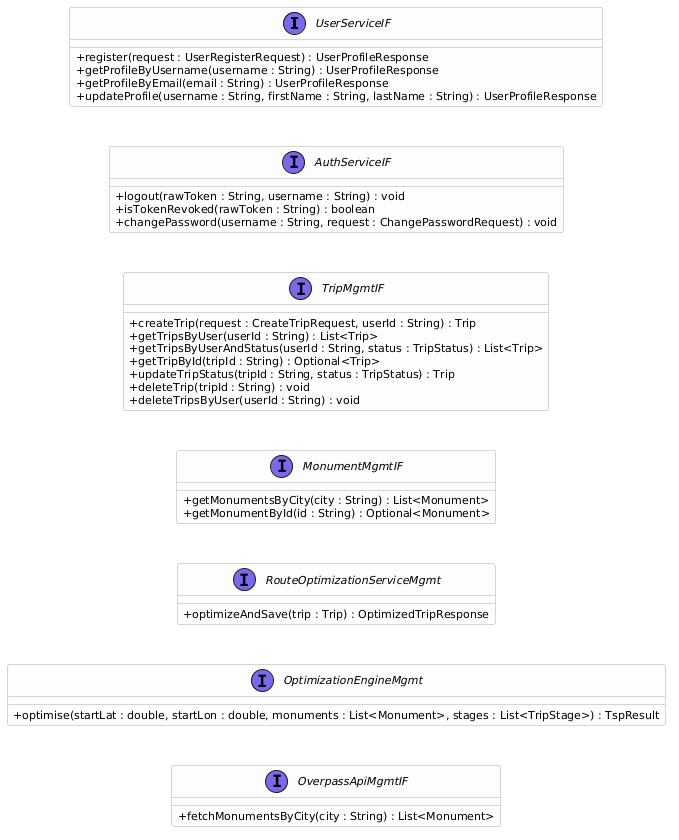
\includegraphics[width=0.75\textwidth]{Iterazione1/Diagrammi/InterfaceDiagram.png}
    \caption{Diagramma delle interfacce}
    \label{fig:IT1InterfaceDiagram}
\end{figure}    

\section{UML Class Diagram}
\begin{figure}[H]
    \centering
    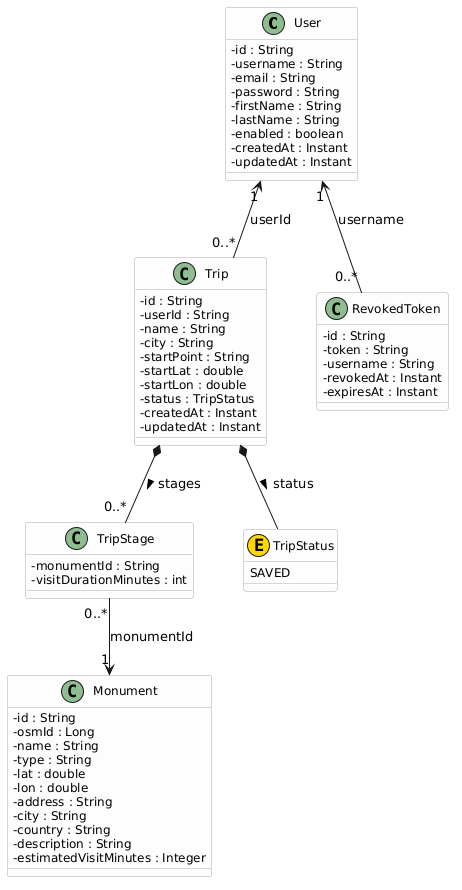
\includegraphics[width=0.7\textwidth]{Iterazione1/Diagrammi/ClassDiagram.png}
    \caption{Diagramma delle classi}
    \label{fig:IT1ClassDiagram}
\end{figure}
\newpage
\section{Component Diagram}

A partire dai casi d’uso, è stata progettata l’architettura del sistema seguendo un’organizzazione a più livelli, al fine di separare chiaramente interfaccia utente, logica applicativa e persistenza dei dati. Questa suddivisione consente di ottenere un sistema modulare ed estendibile.

\begin{figure}[H]
    \centering
    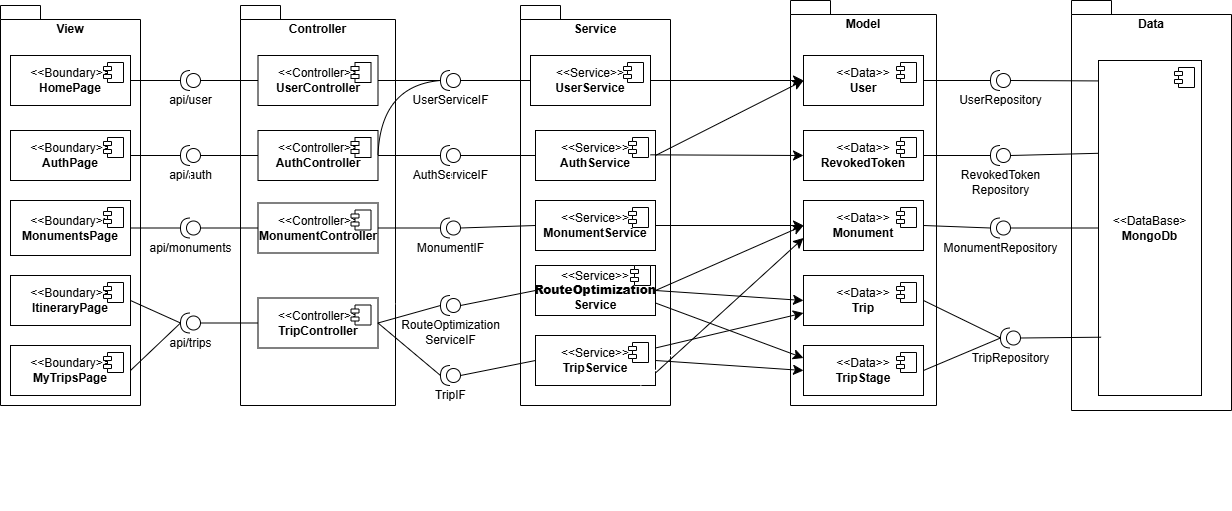
\includegraphics[width=\linewidth]{Iterazione1/Diagrammi/ComponentDiagram.png}
    \caption{Diagramma dei componenti}
    \label{fig:ComponentDiagram}
\end{figure}

Il diagramma è strutturato in cinque livelli principali: \textit{View}, \textit{Controller}, \textit{Service}, \textit{Model} e \textit{Data}. 

\begin{itemize}
    \item \textbf{\textit{View}}: rappresenta i componenti \textit{boundary} del front-end, ovvero le pagine con cui l’utente interagisce direttamente: \textit{HomePage}, \textit{AuthPage}, \textit{MonumentsPage}, \textit{ItineraryPage} e \textit{MyTripsPage}. Questi componenti comunicano con il backend attraverso le API esposte dai controller.
    
    \item \textbf{\textit{Controller}}: contiene i componenti che ricevono le richieste HTTP e le indirizzano verso la logica applicativa appropriata. Il sistema espone endpoint distinti per la gestione degli utenti, dell’autenticazione, dei monumenti e dei viaggi: \textit{UserController}, \textit{AuthController}, \textit{MonumentController} e \textit{TripController}.
    
    \item \textbf{\textit{Service}}: include la logica di business del sistema. I controller delegano a questi componenti l’esecuzione delle operazioni principali attraverso interfacce dedicate, quali \textit{UserServiceIF}, \textit{AuthServiceIF}, \textit{MonumentIF}, \textit{RouteOptimizationServiceIF} e \textit{TripIF}. Le rispettive implementazioni, ovvero \textit{UserService}, \textit{AuthService}, \textit{MonumentService}, \textit{RouteOptimizationService} e \textit{TripService}, si occupano di gestire i dati e le funzionalità del sistema. In particolare, la gestione dei viaggi distingue tra gestione del viaggio e ottimizzazione del percorso.
    
    \item \textbf{\textit{Model}}: definisce le entità del dominio, che rappresentano gli oggetti principali gestiti dall’applicazione: \textit{User}, \textit{RevokedToken}, \textit{Monument}, \textit{Trip} e \textit{TripStage}. Queste classi costituiscono il modello dei dati utilizzato dai service e dal database.
    
    \item \textbf{\textit{Data}}: comprende i componenti responsabili dell’accesso al database, ovvero i repository \textit{UserRepository}, \textit{RevokedTokenRepository}, \textit{MonumentRepository} e \textit{TripRepository}, tutti collegati al database \textit{MongoDb}. Questo livello gestisce le operazioni di lettura e scrittura, mantenendo separata la logica di accesso ai dati dalla logica applicativa.
\end{itemize}

Nel complesso, il diagramma presenta una struttura coerente con il principio di separazione delle responsabilità: le componenti di \textit{View} interagiscono con i \textit{Controller}, i \textit{Controller} delegano ai \textit{Service} la logica di business, i \textit{Service} utilizzano le entità del \textit{Model} e accedono ai dati tramite il livello \textit{Data}. Questa organizzazione rende l’architettura chiara e robusta.
\newpage
\section{Deployment Diagram}

Il seguente deployment diagram rappresenta la distribuzione fisica dei componenti software dell'applicazione all'interno dei diversi nodi di esecuzione.\\
Il sistema è suddiviso in quattro nodi principali: \textit{device, server, database ed external system}. Ogni nodo contiene degli artefatti (file o pacchetti di codice che vengono deployati) e componenti di runtime.\\
Questi nodi interagiscono tra loro mediante opportuni protocolli di comunicazione.

\begin{figure}[H]
    \centering
    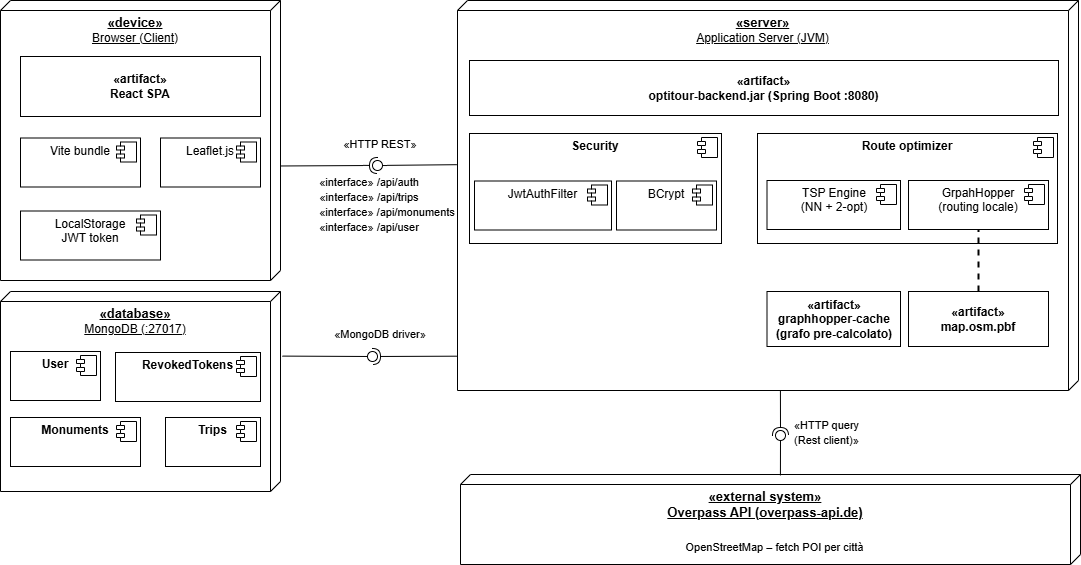
\includegraphics[width=0.75\linewidth]{Iterazione1/Diagrammi/DeploymentDiagram.png}
    \caption{Diagramma di deployment}
    \label{fig:DeploymentDiagram}
\end{figure}

\begin{itemize}
    \item \textbf{Nodo \guillemotleft device\guillemotright \ $\to$ Browser(client):} rappresenta il dispositivo dell'utente finale e contiene l'artefatto: \textbf{React SPA} che a sua volta è composto dal \textit{Vite bundle} e dalla libreria \textit{Leaflet.js} per la visualizzazione delle mappe.\\
    Il browser utilizza inoltre localStorage per memorizzare i JWT token necessari per l'autenticazione delle richieste verso il backend.\\
    La comunicazione verso il nodo server avviene tramite \textbf{HTTP REST } dove il token viene inserito nella header Authorization.
    
    \item \textbf{Nodo \guillemotleft server\guillemotright \ $\to$ Application Server(JVM):} rappresenta l'ambiente di esecuzione del backend basato su \textbf{Spring Boot} e distribuito come:\\
    \textbf{\guillemotleft artifact\guillemotright: optitour-backend.jar:} il quale viene esposto sulla porta :8080.\\
    All'interno del nodo sono presenti i seguenti componenti:
    \begin{itemize}
            \item \textbf{Sicurezza:} intercetta e valida le richieste mediante \textit{JwtAuthFilter} e si occupa dell'hashing delle password tramite \textit{BCrypt}.
            \item \textbf{REST API \ $\to$} esposte tramite gli endpoint: /api/auth, /api/trips,  /api/monuments e /api/user.
            \item \textbf{Motore di ottimizzazione:}
            \begin{itemize}
                \item TPS Engine (Nearest neighbor + 2-opt).
                \item GraphHopper per il routing locale.
            \end{itemize}
            \item  \textbf{Artefatti aggiuntivi}
            \begin{itemize}
                \item \textbf{\guillemotleft artifact\guillemotright map.osm.pbf:} dataset OpenStreetMap.
                \item \textbf{\guillemotleft artifact\guillemotright graphhopper-cache:} grafo pre-calcolato per il routing.
            \end{itemize}
            Il nodo server comunica con MongoDB tramite \textbf{Spring Data MongoDB} e con Overpass API tramite \textbf{HTTP query (REST client)}.
    \end{itemize}
    \item \textbf{Nodo \guillemotleft database\guillemotright \ $\to$ MongoDB:} rappresenta il database NOSQL utilizzato per la persistenza dei dati dell'applicazione.\\
    É esposto sulla porta :27017 e comunica con il backend tramite il driver MongoDB integrato in SpringData.
    \item \textbf{Nodo \guillemotleft eternal system \guillemotright \ $\to$ Overpass API:} rappresenta il sistema esterno basato su OpenStreetMap che viene utilizzato per il recupero dei POI (Point Of Interest) relativi ad una città.
    Il backend interagisce con esso mediante richieste \textbf{HTTP}, utilizzanto un client REST.

\end{itemize}



\newpage
\section{Ottimizzazione del percorso}
\vspace{-5pt} % Riduce spazio sotto il titolo
Dato un insieme di monumenti e un punto di partenza, si cerca un percorso chiuso minimo che visiti tutti i monumenti una sola volta e torni al punto di partenza.
L'algoritmo implementato combina due fasi principali:
\vspace{-5pt}
\begin{enumerate}
    \setlength{\itemsep}{0pt} % Azzera spazio tra i punti
    \setlength{\parskip}{0pt}
    \item \textbf{Heuristica Nearest Neighbour}: costruisce un tour iniziale partendo dal nodo di partenza e visitando il nodo più vicino non ancora visitato.
    \item \textbf{Ottimizzazione 2-opt}: migliora il tour iniziale invertendo coppie di archi quando ciò riduce la distanza totale.
\end{enumerate}

\vspace{-10pt}
\subsection*{Pseudocodice}
\vspace{-5pt}

\begin{algorithm}[H]
\caption{Costruzione matrice delle distanze}
\begin{algorithmic}[1]
\Function{buildDistanceMatrix}{startPoint, monuments}
    \State nodes $\gets$ [startPoint] + monuments, size $\gets$ numero di nodi
    \State dist $\gets$ matrice vuota di dimensione size $\times$ size
    \For{i = 0 \textbf{to} size-1}
        \For{j = 0 \textbf{to} size-1}
            \If{i = j} \State dist[i][j] $\gets 0$
            \Else \State dist[i][j] $\gets$ distanza(nodes[i], nodes[j])
            \EndIf
        \EndFor
    \EndFor
    \State \Return dist
\EndFunction
\end{algorithmic}
\end{algorithm}

\vspace{-15pt} % Salto negativo tra gli algoritmi

\begin{algorithm}[H]
\caption{Nearest Neighbour}
\begin{algorithmic}[1]
\Function{nearestNeighbour}{dist}
    \State size $\gets$ numero di nodi, visited $\gets$ array[size] = false
    \State tour[0] $\gets$ 0, visited[0] $\gets$ true
    \For{step = 1 \textbf{to} size-1}
        \State current $\gets$ tour[step-1], bestNext $\gets$ nodo più vicino non visitato
        \State tour[step] $\gets$ bestNext, visited[bestNext] $\gets$ true
    \EndFor
    \State \Return tour
\EndFunction
\end{algorithmic}
\end{algorithm}

\vspace{-15pt}

\begin{algorithm}[H]
\caption{2-opt}
\begin{algorithmic}[1]
\Function{twoOpt}{tour, dist}
    \State improved $\gets$ true
    \While{improved}
        \State improved $\gets$ false
        \For{i = 0 \textbf{to} size-2}
            \For{j = i+2 \textbf{to} size-1}
                \If{i = 0 \textbf{and} j = size-1} \textbf{continue} \EndIf
                \If{scambio riduce distanza} \State inverti sottosequenza da i+1 a j, improved $\gets$ true
                \EndIf
            \EndFor
        \EndFor
    \EndWhile
    \State \Return tour
\EndFunction
\end{algorithmic}
\end{algorithm}

\subsection*{Analisi della complessità}
\vspace{-5pt}
Nella fase di costruzione della matrice delle distanze, l'algoritmo impiega due cicli annidati per calcolare i percorsi tra tutti i nodi, risultando in una complessità temporale pari a $O(n^2)$, dove $n$ rappresenta il numero totale di nodi (il punto di partenza unito ai monumenti da visitare). Successivamente, l'euristica costruttiva \textit{Nearest Neighbour} valuta, nel caso peggiore, tutti i nodi rimanenti a ogni passo per individuare la destinazione più vicina. Anche in questo caso, la ricerca porta a una complessità temporale di $O(n^2)$. Infine, nella fase di ottimizzazione locale tramite l'algoritmo \textit{2-opt}, vengono confrontate iterativamente coppie di archi nel tentativo di ridurre il costo totale del percorso. Nel caso peggiore, i cicli annidati necessari per queste valutazioni e le relative operazioni di scambio portano a una complessità pari a $O(n^3)$. Di conseguenza, la complessità asintotica totale dell'intero algoritmo è dominata da quest'ultima fase, attestandosi su $O(n^3)$.

\newpage
\section{Test}
In questa sezione vengono descritte le attività di testing, finalizzate alla verifica della qualità e dell’affidabilità del sistema.
\subsection{Test: CodeMR}
L’analisi statica conferma che OptiTour presenta una struttura solida. Il software risulta pulito e privo di componenti critici. L’assenza di “classi problematiche” dimostra che il codice è stato sviluppato con cura, mantenendo ogni modulo isolato e facilmente gestibile. Questo garantisce che il sistema sia semplice da manutenere e pronto per le iterazioni successive del progetto.

\begin{figure}[H]
    \centering
    % --- 2. COMPLESSITÀ ---
    \begin{minipage}[b]{0.32\textwidth}
        \centering
        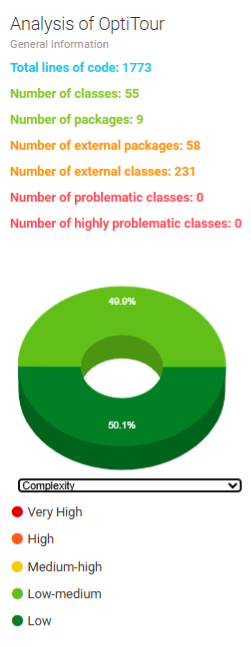
\includegraphics[width=\textwidth]{Iterazione1/Diagrammi/codeMR/complessità.png}
        \caption{Analisi della complessità.}
        \label{fig:IT1_Complexity_MVC}
    \end{minipage}
    \hfill
    % --- 3. ACCOPPIAMENTO ---
    \begin{minipage}[b]{0.32\textwidth}
        \centering
        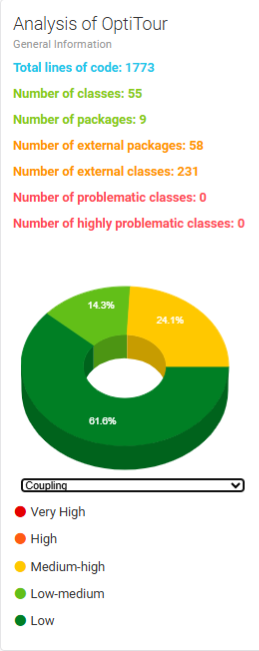
\includegraphics[width=\textwidth]{Iterazione1/Diagrammi/codeMR/Accoppiamento.png}
        \caption{Grado di accoppiamento.}
        \label{fig:IT1_Coupling_MVC}
    \end{minipage}
    \hfill
    % --- 4. COESIONE ---
    \begin{minipage}[b]{0.32\textwidth}
        \centering
        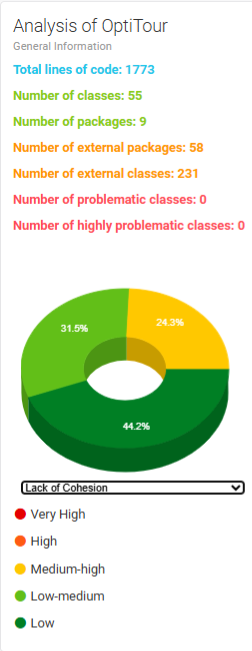
\includegraphics[width=\textwidth]{Iterazione1/Diagrammi/codeMR/MancanzaCoesione.png}
        \caption{Livello di coesione.}
        \label{fig:IT1_Cohesion_MVC}
    \end{minipage}
\end{figure}
% --- 1. STRUTTURA DEI PACKAGE ---
\begin{figure}[H]
    \centering
    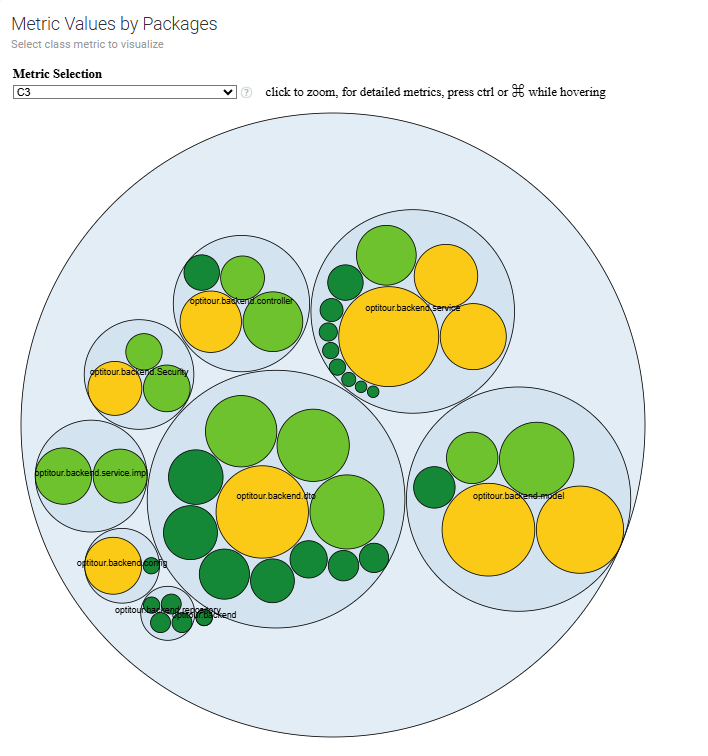
\includegraphics[width=0.8\textwidth]{Iterazione1/Diagrammi/codeMR/StrutturaPackage.png}
    \caption{Distribuzione dei componenti: organizzazione delle classi nei package Model, View/DTO, Service e Controller.}
    \label{fig:IT1_MVC_Structure}
\end{figure}


\newpage
\subsection{Test: Junit}
\newpage
\chapter{Iterazione 2}
\section{Casi d'uso implementati}
In questa seconda fase di sviluppo, l'attenzione si è concentrata sull'estensione delle funzionalità di gestione dei viaggi, con particolare riguardo alla condivisione e alla modifica granulare degli itinerari. Sono stati implementati il catalogo pubblico (con la relativa funzione di pubblicazione), lo storico, la gestione dei percorsi salvati/preferiti e la possibilità di eliminare singole tappe. Di seguito sono riportati i casi d'uso sviluppati per questa iterazione, in conformità con i requisiti iniziali.

\begin{table}[htbp]
\centering
\renewcommand{\arraystretch}{1.2}
\begin{tabular}{|l|l|}
\hline
\textbf{ID} & \textbf{Titolo} \\
\hline
UC3.1 & Visualizza catalogo \\
\hline
UC3.3 & Visualizza storico \\
\hline
UC4 & Filtri ricerca \\
\hline
UC5 & Salva percorso nei preferiti \\
\hline
UC7 & Rimuovi percorso salvato \\
\hline
UC8 & Pubblica percorso nel catalogo \\
\hline
UC10 & Imposta percorso completato \\
\hline
UC12.2 & Creazione itinerario casuale \\
\hline
UC15 & Modifica tappe \\
\hline
UC16 & Elimina tappa \\
\hline
\end{tabular}
\caption{Iterazione 2 - Casi d'uso implementati}
\label{tab:casi_uso_iterazione2}
\end{table}

\subsection*{UC3.1: Visualizza catalogo}
\textbf{Attori:} Utente, Sistema.\\
\textbf{Descrizione:} L'utente può visualizzare percorsi creati da altri utenti e resi pubblici, raccolti all'interno di un catalogo condiviso.\\
\textbf{Flusso degli eventi:}
\begin{enumerate}
    \item L'utente accede alla sezione "Catalogo" tramite l'interfaccia principale.
    \item Il sistema recupera dal database la lista dei viaggi con visibilità pubblica.
    \item Il sistema mostra all'utente l'elenco dei viaggi disponibili.
    \item L'utente può selezionare un singolo viaggio per visualizzarne i dettagli.
\end{enumerate}

\subsection*{UC3.3: Visualizza storico}
\textbf{Attori:} Utente, Sistema.\\
\textbf{Descrizione:} L'utente può consultare l'elenco dei propri viaggi passati, contrassegnati come completati.\\
\textbf{Flusso degli eventi:}
\begin{enumerate}
    \item L'utente accede alla sezione "Storico" dal proprio profilo.
    \item Il sistema interroga il database filtrando i viaggi dell'utente con stato \texttt{COMPLETED}.
    \item Il sistema restituisce e mostra a schermo l'elenco dei percorsi effettuati.
\end{enumerate}

\subsection*{UC4: Filtri ricerca}
\textbf{Attori:} Utente, Sistema.\\
\textbf{Descrizione:} L'utente può filtrare i percorsi nel catalogo in base a criteri quali città, durata massima o numero di tappe.\\
\textbf{Flusso degli eventi:}
\begin{enumerate}
    \item L'utente imposta i parametri del filtro nella sezione Catalogo.
    \item L'utente avvia la ricerca.
    \item Il sistema applica i filtri tramite una query su MongoDB.
    \item La vista viene aggiornata mostrando solo i risultati pertinenti.
\end{enumerate}

\subsection*{UC5: Salva percorso nei preferiti}
\textbf{Attori:} Utente, Sistema.\\
\textbf{Descrizione:} L'utente può aggiungere un percorso di interesse alla propria sezione dei preferiti.\\
\textbf{Flusso degli eventi:}
\begin{enumerate}
    \item L'utente visualizza un viaggio dal Catalogo o dai propri viaggi.
    \item Seleziona l'opzione di salvataggio nei preferiti.
    \item Il sistema crea l'associazione nel database.
    \item Il sistema conferma l'avvenuto salvataggio.
\end{enumerate}

\subsection*{UC7: Rimuovi percorso salvato}
\textbf{Attori:} Utente, Sistema.\\
\textbf{Descrizione:} L'utente può rimuovere un itinerario precedentemente salvato nella propria area personale.\\
\textbf{Flusso degli eventi:}
\begin{enumerate}
    \item L'utente accede alla sezione dei percorsi salvati.
    \item Seleziona il viaggio da rimuovere.
    \item Il sistema elimina l'associazione nel database.
    \item La lista viene aggiornata rimuovendo l'elemento dall'interfaccia.
\end{enumerate}

\subsection*{UC8: Pubblica percorso nel catalogo}
\textbf{Attori:} Utente, Sistema.\\
\textbf{Descrizione:} L'utente rende pubblico un proprio viaggio, permettendo ad altri utenti di visualizzarlo nel catalogo.\\
\textbf{Flusso degli eventi:}
\begin{enumerate}
    \item L'utente apre i dettagli di un proprio viaggio salvato.
    \item Seleziona l'opzione "Pubblica nel catalogo".
    \item Il sistema aggiorna lo stato di visibilità dell'itinerario nel database.
    \item Il percorso diventa visibile a tutti gli utenti nella sezione Catalogo.
\end{enumerate}

\subsection*{UC10: Imposta percorso completato}
\textbf{Attori:} Utente, Sistema.\\
\textbf{Descrizione:} L'utente contrassegna un viaggio come completato al termine della visita.\\
\textbf{Flusso degli eventi:}
\begin{enumerate}
    \item L'utente seleziona un viaggio attivo.
    \item Clicca su "Segna come completato".
    \item Il sistema aggiorna lo stato in \texttt{COMPLETED}.
    \item Il viaggio viene spostato automaticamente nella sezione Storico.
\end{enumerate}

\subsection*{UC12.2: Creazione itinerario casuale}
\textbf{Attori:} Utente, Sistema.\\
\textbf{Descrizione:} Generazione automatica di un itinerario basato su parametri casuali (città e numero tappe).\\
\textbf{Flusso degli eventi:}
\begin{enumerate}
    \item L'utente richiede un viaggio casuale specificando la città.
    \item Il sistema recupera i POI (da database o Overpass API).
    \item Il sistema seleziona un set casuale di monumenti rispettando i vincoli.
    \item Viene generato e mostrato il percorso ottimizzato sulla mappa.
\end{enumerate}

\subsection*{UC15: Modifica tappe}
\textbf{Attori:} Utente, Sistema.\\
\textbf{Descrizione:} L'utente modifica un viaggio esistente aggiungendo nuovi monumenti e richiedendo il ricalcolo dell'itinerario.\\
\textbf{Flusso degli eventi:}
\begin{enumerate}
    \item L'utente apre un viaggio in modalità modifica.
    \item Aggiunge una o più tappe selezionandole dalla mappa o dalla lista.
    \item Il sistema invoca l'Optimization Engine per ricalcolare il percorso TSP.
    \item Il viaggio aggiornato viene salvato con i nuovi dati di tempo e distanza.
\end{enumerate}

\subsection*{UC16: Elimina tappa}
\textbf{Attori:} Utente, Sistema.\\
\textbf{Descrizione:} L'utente può rimuovere una singola tappa da un itinerario esistente.\\
\textbf{Flusso degli eventi:}
\begin{enumerate}
    \item L'utente apre i dettagli di un viaggio salvato.
    \item Identifica la tappa da rimuovere e seleziona l'opzione di eliminazione.
    \item Il sistema rimuove la tappa dalla lista e ricalcola immediatamente l'ottimizzazione del percorso rimanente.
    \item L'interfaccia aggiorna la mappa e i dettagli del viaggio.
\end{enumerate}
\newpage
\section{Diagramma delle interfacce}
\begin{figure}[H]
    \centering
    \includegraphics[width=0.9\textwidth]{Iterazione2/Diagrammi/InterfaceDiagram2.png}
    \caption{Diagramma delle interfacce - Iterazione 2.}
    \label{fig:interface_diagram2}
\end{figure}
Il diagramma in Figura \autoref{fig:interface_diagram2} illustra le interfacce aggiornate del sistema per la seconda iterazione. Rispetto alla fase precedente, sono state ampliate le firme dei metodi nei service, in particolare all'interno di \texttt{TripMgmtIF}, per supportare nativamente le nuove funzionalità legate al recupero dei viaggi pubblici (catalogo), alla gestione dello storico, dei preferiti e all'aggiormanento di un viaggio con la conseguente rimozione/aggiunta di tappe e modifica di durata di visita.

\newpage
\section{UML Class Diagram}
\begin{figure}[H]
    \centering
    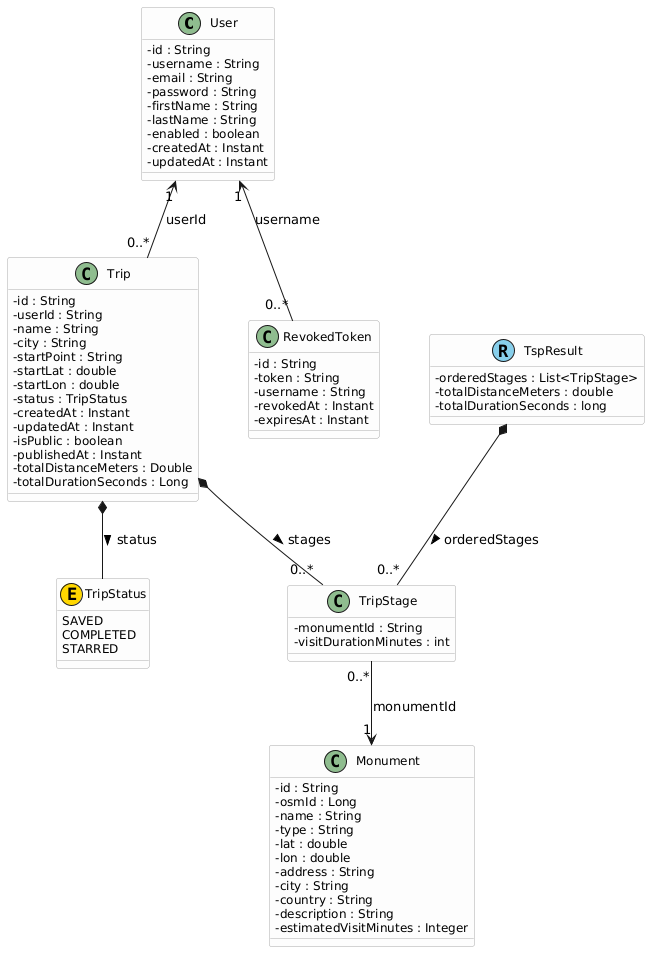
\includegraphics[width=0.85\textwidth]{Iterazione2/Diagrammi/ClassDiagram2.png}
    \caption{UML Class Diagram - Iterazione 2.}
    \label{fig:class_diagram_2}
\end{figure}

Il diagramma delle classi (\autoref{fig:class_diagram2}) mostra l'evoluzione del modello dati nella seconda iterazione. L'entità principale \texttt{Trip} è stata arricchita per poter gestire il nuovo ciclo di vita dei percorsi:
\begin{itemize}
    \item L'enumerazione \texttt{TripStatus} ora include i nuovi stati \texttt{COMPLETED} (per lo storico) e \texttt{STARRED} (per i preferiti), oltre a \texttt{SAVED} già introdotto nella fase precedente.
    \item Sono stati aggiunti gli attributi \texttt{isPublic} e \texttt{publishedAt} per gestire la visibilità dei viaggi all'interno del catalogo condiviso.
\end{itemize}

\newpage
\section{Component Diagram}

Rispetto alla precedente iterazione, l’architettura del sistema è stata estesa mantenendo invariata la struttura a più livelli già adottata. In questo modo è stata conservata la separazione tra interfaccia utente, logica applicativa e gestione dei dati, introducendo però nuove funzionalità lato front-end e ampliando i componenti esistenti.

\begin{figure}[H]
    \centering
    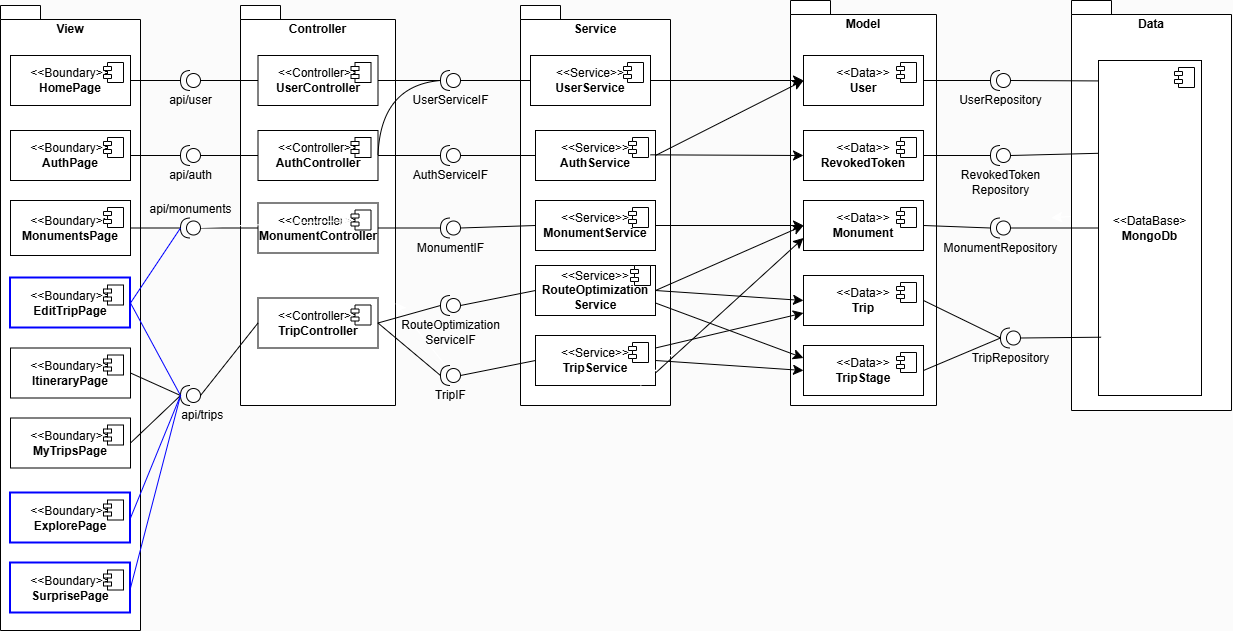
\includegraphics[width=\linewidth]{Iterazione2/Diagrammi/ComponentDiagramIt2.png}
    \caption{Diagramma dei componenti}
    \label{fig:ComponentDiagramIterazione2}
\end{figure}

In questa iterazione sono state aggiunte tre nuove pagine nel livello \textit{View}, ovvero \textit{ExplorePage}, \textit{SurprisePage} ed \textit{EditTripPage}. Gli altri livelli non introducono nuove classi, ma sono stati ampliati nelle funzionalità interne per supportare i nuovi casi d’uso e le nuove interazioni dell’applicazione.

Il diagramma mostra quindi un’evoluzione coerente dell’architettura: le nuove pagine del front-end sfruttano i controller esistenti, che delegano ai service aggiornati, i quali operano sulle entità del \textit{Model} e accedono ai dati attraverso il livello \textit{Data}. 
\newpage
\section{Deployment diagram}
\vspace{0.5cm}

\begin{figure}[H]
    \centering
    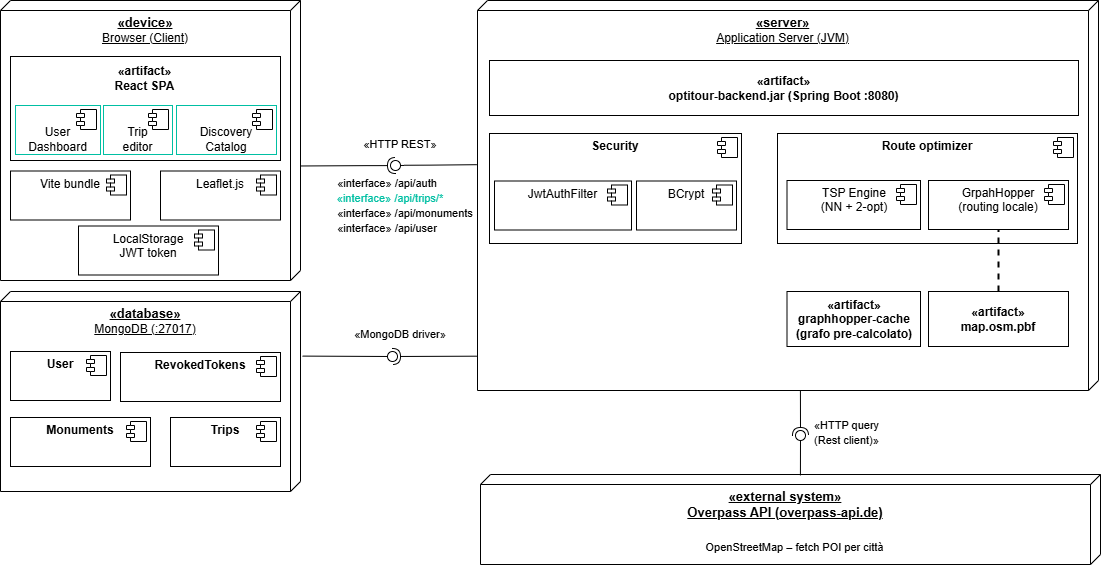
\includegraphics[width=0.85\textwidth]{Iterazione2/Diagrammi/DeploymentDiagram2.png}
    \caption{Diagramma di deployment}
    \label{fig:class_diagram2}
\end{figure}

Il diagramma di deployment è stato aggiornato per rappresentare le evoluzioni architetturali necessarie a supportare i nuovi casi d’uso dell’applicazione.\\
Come mostrato nel diagramma, tali modifiche non hanno richiesto l’introduzione di nuovi nodi fisici o di ulteriori database, ma hanno comportato un ampliamento dei moduli logici già presenti negli artefatti esistenti.

Per quanto riguarda l’interazione con l’utente, all’interno dell’artefatto \texttt{React SPA}, collocato nel nodo \textit{Browser (Client)}, sono stati definiti tre nuovi macro-componenti software che raccolgono la logica applicativa relativa ai seguenti Use Case (UC):

\begin{itemize}
    \item \textbf{User Dashboard}: gestisce l’area personale dell’utente e il monitoraggio dei suoi itinerari. Include i casi d’uso relativi alle preferenze e allo stato dei percorsi, ovvero \textit{UC3.3 (Visualizza storico)}, \textit{UC5 (Salva percorso nei preferiti)}, \textit{UC7 (Rimuovi percorso salvato)} e \textit{UC10 (Imposta percorso completato)}.

    \item \textbf{Trip editor}: modulo dedicato alla modifica degli itinerari esistenti. Implementa le funzionalità richieste dall’utente per aggiornare o rimuovere tappe, in particolare \textit{UC15 (Modifica tappe)} e \textit{UC16 (Elimina tappa)}.

    \item \textbf{Discovery Catalog}: componente orientato alla consultazione e alla scoperta di nuovi percorsi. Fornisce l’interfaccia per il catalogo pubblico (\textit{UC3.1 Visualizza catalogo}, \textit{UC8 Pubblica percorso nel catalogo}), per i filtri di ricerca (\textit{UC4 Filtri ricerca}) e per la generazione di itinerari casuali (\textit{UC12.2 Creazione itinerario casuale}).
\end{itemize}

Dal lato server, nel nodo \textit{Application Server (JVM)}, l’integrazione di queste funzionalità ha richiesto un’estensione dell’interfaccia \textbf{REST API}.\\
Nel diagramma, l’endpoint principale è stato generalizzato come \texttt{«interface» /api/trips/*} per indicare in modo formale l’esposizione dei nuovi sotto-percorsi (ad esempio: \texttt{/history}, \texttt{/catalog}, \texttt{/random}, \texttt{/\{id\}/save}) necessari a gestire le richieste HTTP provenienti dai moduli frontend introdotti.

\vspace{0.5cm}

\newpage
\section{Test}
In questa sezione vengono descritte le attività di testing svolte durante questa iterazione, con l’obiettivo di verificare la correttezza, l’affidabilità e la stabilità delle nuove funzionalità introdotte. I test sono stati condotti sia a livello di singoli componenti, per validare la logica di business, sia a livello di integrazione, per assicurare il corretto funzionamento delle API esposte e la comunicazione tra frontend e backend. Particolare attenzione è stata dedicata alla verifica degli endpoint relativi alla gestione dei viaggi e delle nuove funzionalità introdotte, includendo operazioni di visualizzazione del catalogo pubblico, consultazione dello storico, applicazione dei filtri di ricerca, gestione dei percorsi preferiti e aggiornamento dello stato dei viaggi come completati. Sono state inoltre testate le funzionalità di creazione di itinerari casuali e di modifica delle tappe, comprensive del ricalcolo del percorso ottimizzato tramite il motore TSP.
\subsection{Test: CodeMR}
L'analisi statica del codice per la seconda iterazione è stata condotta tramite CodeMR. Rispetto all'iterazione precedente, le metriche riflettono la naturale espansione del sistema: le linee di codice totali sono aumentate e il numero di classi anche. Nonostante l'introduzione di numerose funzionalità (catalogo pubblico, storico, filtri e percorsi casuali), l'architettura mantiene un livello di qualità elevato, registrando zero classi "altamente problematiche" e solo tre classi "problematiche".
Di seguito vengono analizzate le tre metriche principali: Complessità, Accoppiamento e Mancanza di Coesione.

\begin{figure}
    \centering
    \begin{minipage}{0.30\textwidth}
        \centering
        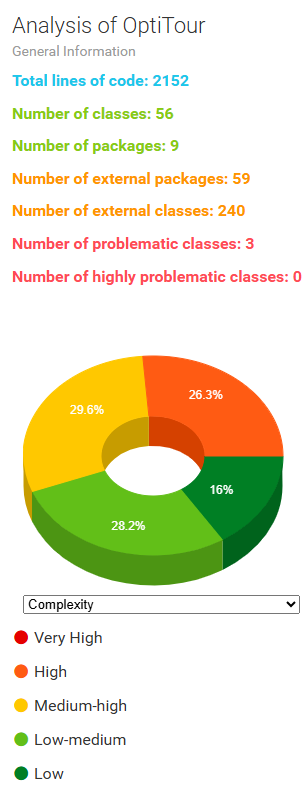
\includegraphics[width=\textwidth]{Iterazione2/Diagrammi/codeMR/complexityIT2.png}
        \caption{Complessità.}
        \label{fig:codemr_complexity}
    \end{minipage}\hfill
    \begin{minipage}{0.30\textwidth}
        \centering
        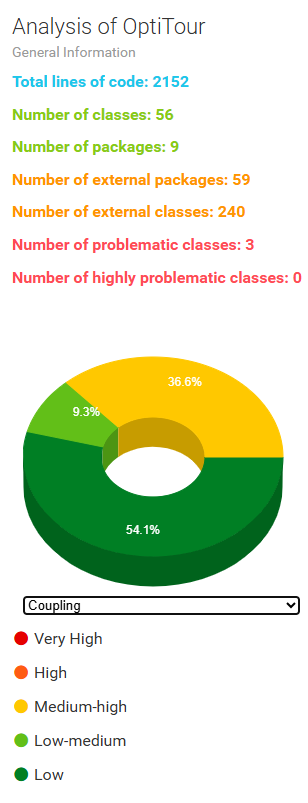
\includegraphics[width=\textwidth]{Iterazione2/Diagrammi/codeMR/CouplingIT2.png}
        \caption{Accoppiamento.}
        \label{fig:codemr_coupling}
    \end{minipage}\hfill
    \begin{minipage}{0.30\textwidth}
        \centering
        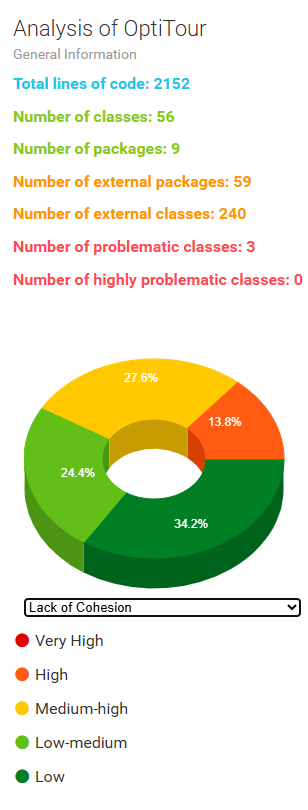
\includegraphics[width=\textwidth]{Iterazione2/Diagrammi/codeMR/CoesioneIT2.png}
        \caption{Lack of Cohesion.}
        \label{fig:codemr_cohesion}
    \end{minipage}
\end{figure}

\begin{itemize}
    \item \textbf{Complessità:} L'aggiunta di logiche avanzate ha comportato un fisiologico aumento della complessità in alcune classi. Tuttavia, la maggior parte del sistema si mantiene su livelli bassi o medio-bassi.
    \item \textbf{Accoppiamento:} I risultati confermano l'efficacia dell'architettura a livelli (MVC) e dell'uso delle interfacce. Oltre il 54\% delle classi ha un livello di accoppiamento "Basso" e non si registrano classi nella fascia "Alta" o "Molto Alta".
    \item \textbf{Coesione:} La distribuzione rimane bilanciata. Una buona porzione del sistema mostra un'alta coesione (indicata dai valori bassi/verdi di "Lack of Cohesion"), sinonimo di classi robuste, con responsabilità singole ben definite e facili da manutenere.
\end{itemize}

\subsubsection*{Analisi delle Classi Complesse e Struttura dei Package}
L'analisi di dettaglio ha evidenziato che la classe con il maggior grado di complessità è il \texttt{TripService} (\autoref{fig:classe_complex}). Questo risultato è ampiamente giustificato: come dimostrato anche nei test JUnit, il \texttt{TripService} funge da gestore centrale della logica di business, gestendo le validazioni, la sicurezza, la storicizzazione, il ricalcolo del TSP e l'integrazione con i database per tutto il ciclo di vita dei viaggi. L'accoppiamento e la mancanza di coesione per questa classe rimangono comunque nella fascia media.
\begin{figure}
    \centering
    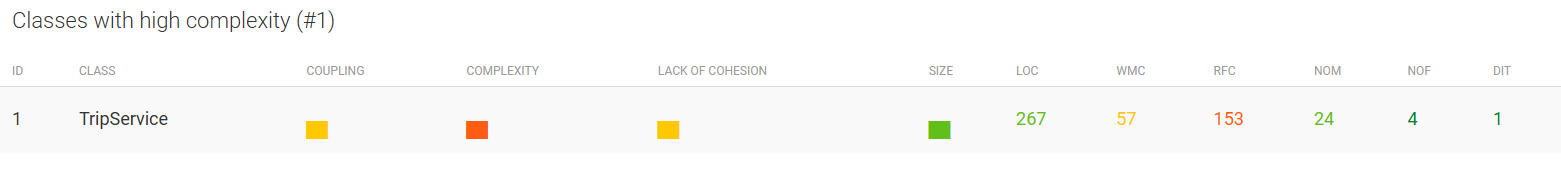
\includegraphics[width=0.7\textwidth]{Iterazione2/Diagrammi/codeMR/ClasseAltaComplex.png}
    \caption{Dettaglio della classe TripService, identificata con complessità alta.}
    \label{fig:classe_complex}
\end{figure}
Infine, la visualizzazione della metrica strutturale per package (\autoref{fig:struttura_codemr}) conferma che i pesi maggiori in termini di dimensioni e complessità risiedono nei layer \texttt{service}, \texttt{model} e \texttt{dto}. Al contrario, il layer \texttt{controller} mantiene dimensioni più contenute, limitandosi correttamente a intercettare e instradare le chiamate esterne senza inglobare logica applicativa.
\begin{figure}
    \centering
    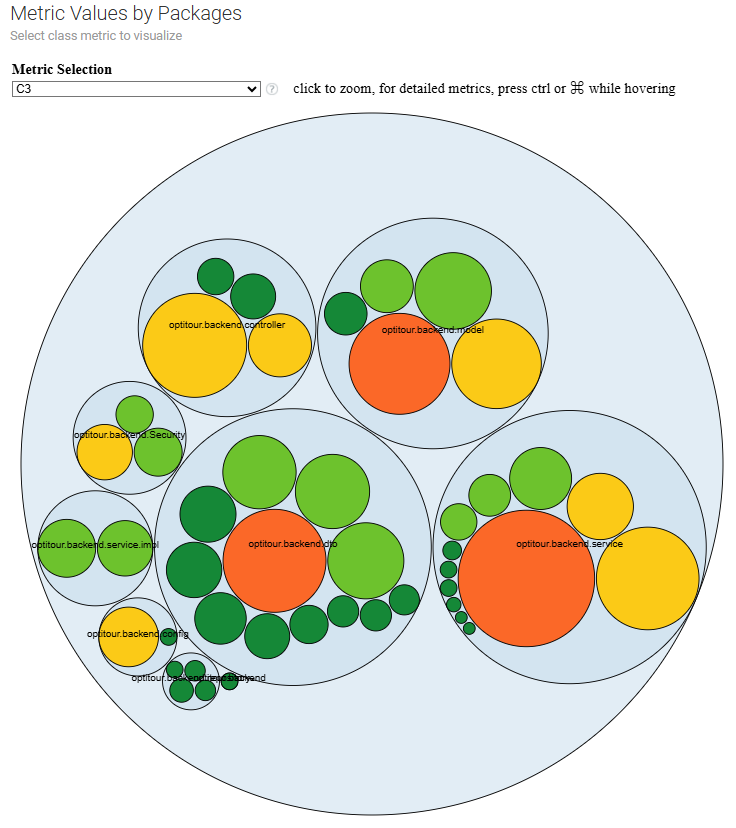
\includegraphics[width=0.7\textwidth]{Iterazione2/Diagrammi/codeMR/strutturaIT2.png}
    \caption{Distribuzione delle metriche all'interno dei package architetturali.}
    \label{fig:struttura_codemr}
\end{figure}

\newpage
\subsection{Test: Junit}
Questa sezione è dedicata ai test eseguiti con JUnit. La copertura dei test riguardanti l'autenticazione base, la gestione degli utenti, l'integrazione con le API dei monumenti e l'algoritmo centrale del TSP è rimasta inalterata rispetto all'Iterazione 1, risultando quindi già del tutto validata.

\subsubsection*{1. Sicurezza e Validazione Token}
 Sono stati aggiunti test specifici per il livello di sicurezza, questi nuovi moduli verificano la corretta autorizzazione delle richieste HTTP tramite i filtri JWT, gestendo casi limite come l'uso di token malformati, revocati o scaduti (\autoref{fig:auth_test} e  \autoref{fig:token_test}), oltre a validare la logica di estrazione dei dettagli utente dal database ( \autoref{fig:custom_detail_test}).

\begin{figure}[H]
    \centering
    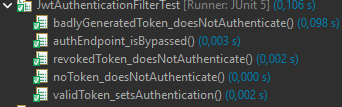
\includegraphics[width=0.7\textwidth]{Iterazione2/Diagrammi/test/AuthTest.png}
    \caption{Test del filtro di autenticazione JWT e gestione dei token.}
    \label{fig:auth_test}
\end{figure}
\begin{figure}[H]
    \centering
    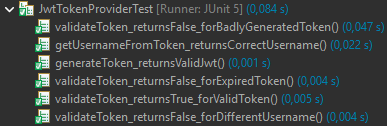
\includegraphics[width=0.7\textwidth]{Iterazione2/Diagrammi/test/TokenTest.png}
    \caption{Validazione del Provider JWT.}
    \label{fig:token_test}
\end{figure}
\begin{figure}[H]
    \centering
    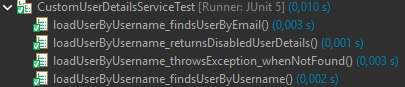
\includegraphics[width=0.7\textwidth]{Iterazione2/Diagrammi/test/CustomDetailService.png}
    \caption{Test del Custom User Details Service.}
    \label{fig:custom_detail_test}
\end{figure}


\subsubsection*{2. Gestione Viaggi (TripService e TripController)}
Il cuore del lavoro di testing di questa iterazione si è concentrato sull'espansione dei controller e dei service legati ai viaggi, che ora coprono un vasto ventaglio di nuovi casi d'uso. Come viene mostrato in \autoref{fig:trip_controller_test}, i test a livello di Controller validano l'esposizione delle nuove API per il recupero dei viaggi pubblici (catalogo), l'applicazione di filtri case-insensitive per città e la corretta gestione degli stati del viaggio (salvataggio nei preferiti, completamento, ripristino).

\begin{figure}
    \centering
    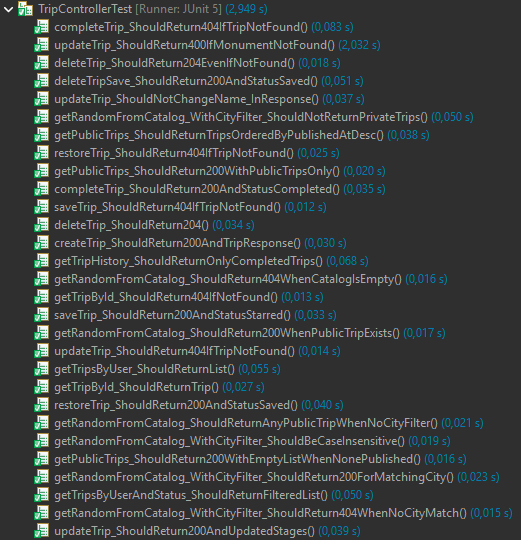
\includegraphics[width=0.9\textwidth]{Iterazione2/Diagrammi/test/TripControllerTest.png}
    \caption{Espansione dei test sugli endpoint del TripController.}
    \label{fig:trip_controller_test}
\end{figure}

A livello di logica di business, il \texttt{TripServiceTest} (\autoref{fig:trip_service_test}) è stato arricchito per validare rigorosamente le regole applicative. I test assicurano che:
\begin{itemize}
    \item La generazione casuale dei viaggi rispetti i vincoli imposti.
    \item Vengano applicati rigorosi controlli di sicurezza (es. eccezione 403 Forbidden se un utente tenta di modificare o pubblicare un viaggio non suo).
    \item I flussi di pubblicazione (IsPublic) e la storicizzazione funzionino in stretta sinergia con il database.
\end{itemize}

\begin{figure}
    \centering
    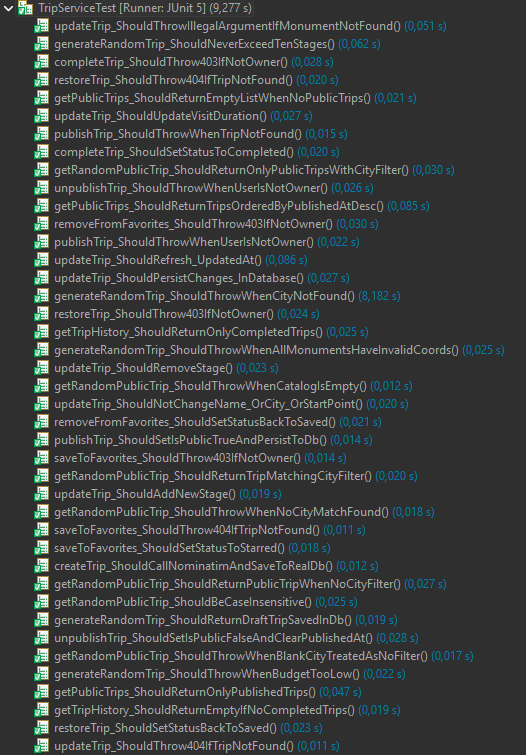
\includegraphics[width=0.8\textwidth]{Iterazione2/Diagrammi/test/TripServiceTest.png}
    \caption{Espansione dei test della logica di business nel TripServiceTest.}
    \label{fig:trip_service_test}
\end{figure}

\newpage
\subsection{API Esposte}

In questa sezione vengono descritte le principali API esposte dal backend tramite i controller di Spring Boot, necessarie per supportare i casi d’uso sviluppati e testate tramite Postman.

\begin{enumerate}

\item \textbf{Gestione Viaggi}

\textbf{Aggiornamento di un Viaggio}

\begin{itemize}
    \item \textbf{Endpoint:} PUT /api/trips/\{id\}

    \item \textbf{Descrizione:} Permette di aggiornare un viaggio esistente modificandone le informazioni principali, come la durata per ciascuna tappa, l’aggiunta e la rimozione di tappe con le relative tempistiche. 
    I dettagli della richiesta e della risposta sono illustrati in \autoref{fig:updateTripRequest} e Figura \autoref{fig:updateTripResponse}.

    \item \textbf{Parametri:}
    \begin{itemize}
        \item \{id\} (string) - ID del viaggio da aggiornare.
    \end{itemize}

    \item \textbf{Payload:}
    \begin{itemize}
        \item name (string) - Nome del viaggio.
        \item city (string) - Città del viaggio.
        \item startPoint (string) - Punto di partenza.
        \item stages (array) - Lista aggiornata delle tappe del viaggio.
    \end{itemize}

\end{itemize}

\end{enumerate}

\begin{figure}[H]
    \centering
    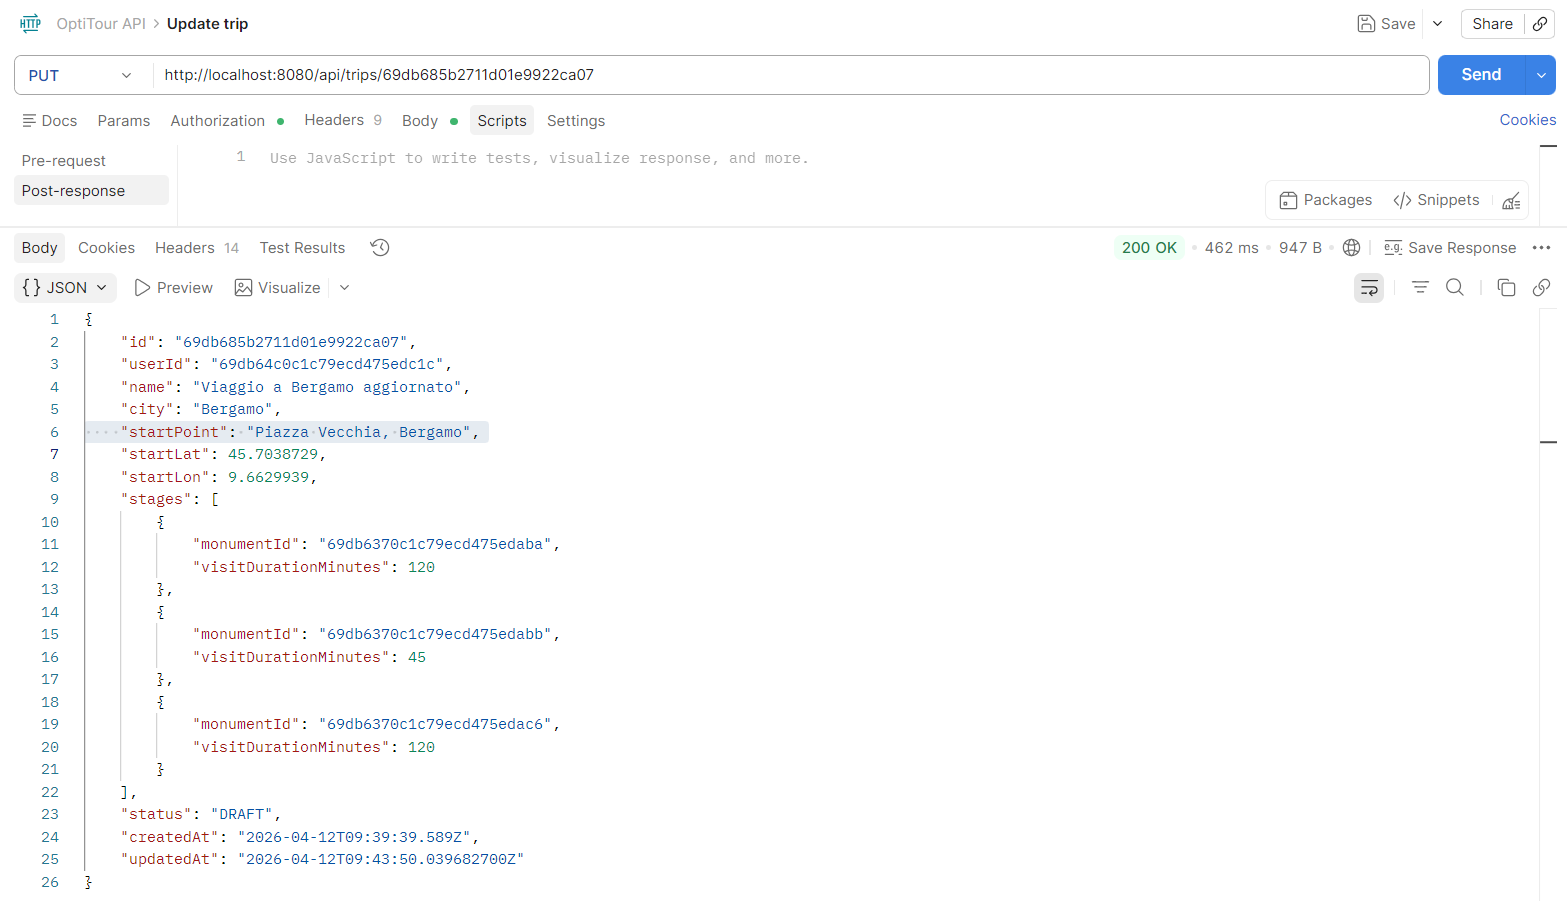
\includegraphics[width=0.8\textwidth]{Iterazione2/Diagrammi/API/updateTripApi.png}
    \caption{Test su Postman: Payload di richiesta per l’aggiornamento di un viaggio.}
    \label{fig:updateTripRequest}
\end{figure}

\begin{figure}[H]
    \centering
    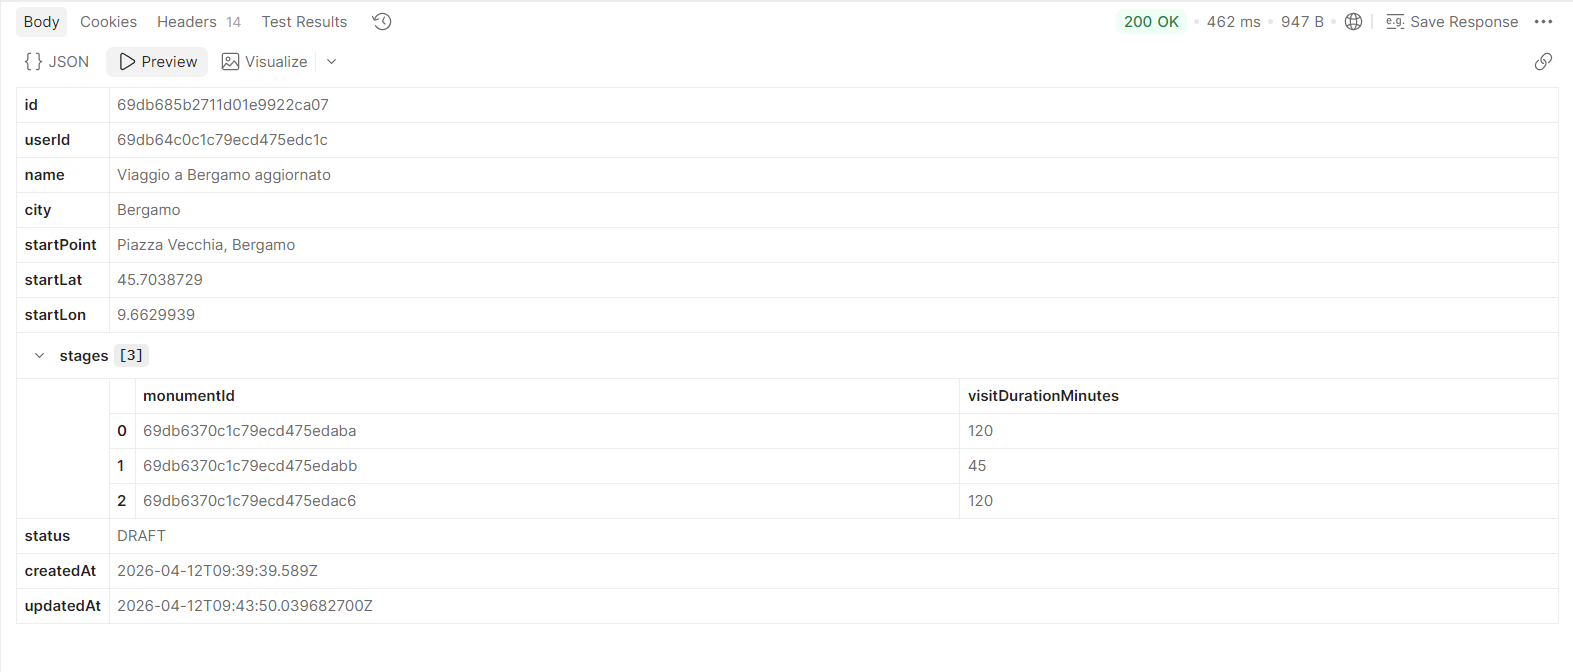
\includegraphics[width=0.8\textwidth]{Iterazione2/Diagrammi/API/updateTripApiResponse.png}
    \caption{Test su Postman: Risposta del server dopo l’aggiornamento del viaggio.}
    \label{fig:updateTripResponse}
\end{figure}


\newpage
%\chapter{Iterazione 3}


%\input{conclusione}
%\addcontentsline{toc}{chapter}{Conclusione} % Aggiunge al sommario
%\markboth{Conclusione}{Conclusione}         % <--- AGGIUNGI QUESTO
% =========== Bibliografia =========== %

%\bibliographystyle{unsrt}
%\bibliography{references}

\end{document}


